\subsection{Gantt Chart}

This Gantt chart details the sequence of activities scheduled for the eight sprints over the duration of the FYP, highlighting the start and end weeks for each module's development and indicating any overlapping activities \cite{gantt1}. Each sprint consists of a four-week period. This chart facilitates quick comprehension of the timeline, allowing us to verify that the requirements definition phase concludes before implementation begins and that the testing phase commences early enough to identify and rectify any integration issues prior to the final sprint. The complete timeline is illustrated in Figure~\ref{fig:ganttchart}.

\begin{figure}[H]
\centering
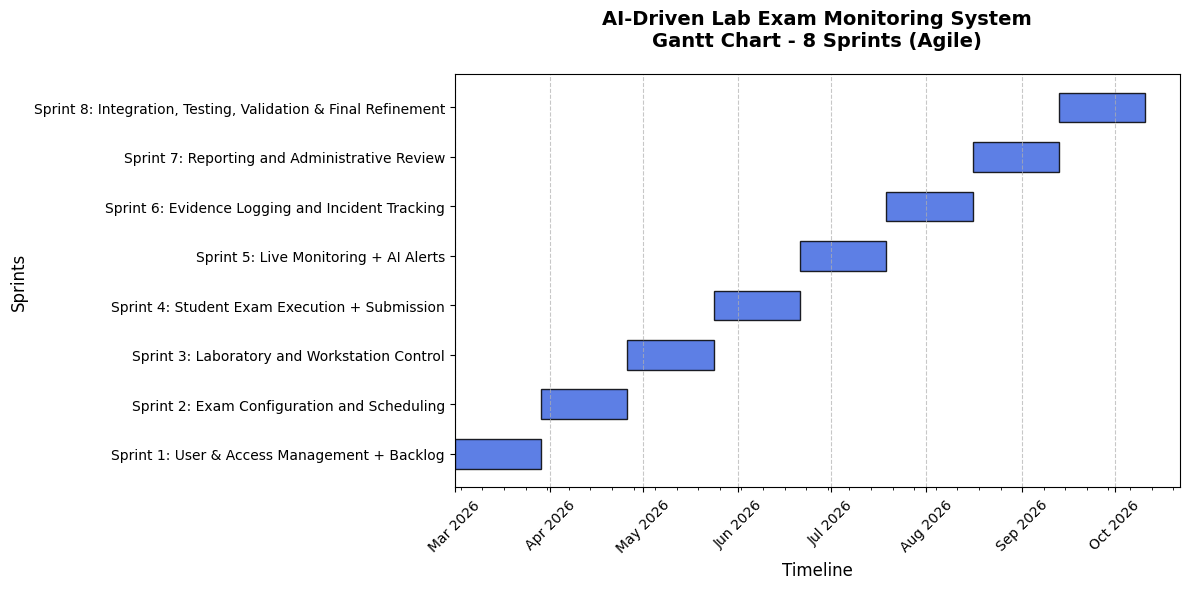
\includegraphics[width=0.95\linewidth]{Figures/gantt_chart.png}
\caption{Project Gantt Chart Based on Eight Agile Sprints}
\label{fig:ganttchart}
\end{figure}

Our understanding of the Gantt chart in Figure~\ref{fig:ganttchart} should align with the detailed sprint descriptions provided in Chapter 1.8. Each block of the chart represents the tasks performed within a sprint iteration, not a strict waterfall model. Any critical issues found during a sprint review will lead to an update of the Gantt chart before the next sprint commences \cite{spp1}.

\subsection{Work Breakdown Structure}

The Work Breakdown Structure (WBS) systematically deconstructs the project into manageable work packages \cite{wbs1}. Initially, the project is divided into five core areas: Requirements, Design, Implementation, Testing, and Documentation. Subsequently, the implementation phase is further segmented to encompass the twelve module clusters defined in the product scope. Figure~\ref{fig:wbs} outlines the full hierarchical structure.

\begin{figure}[H]
\centering
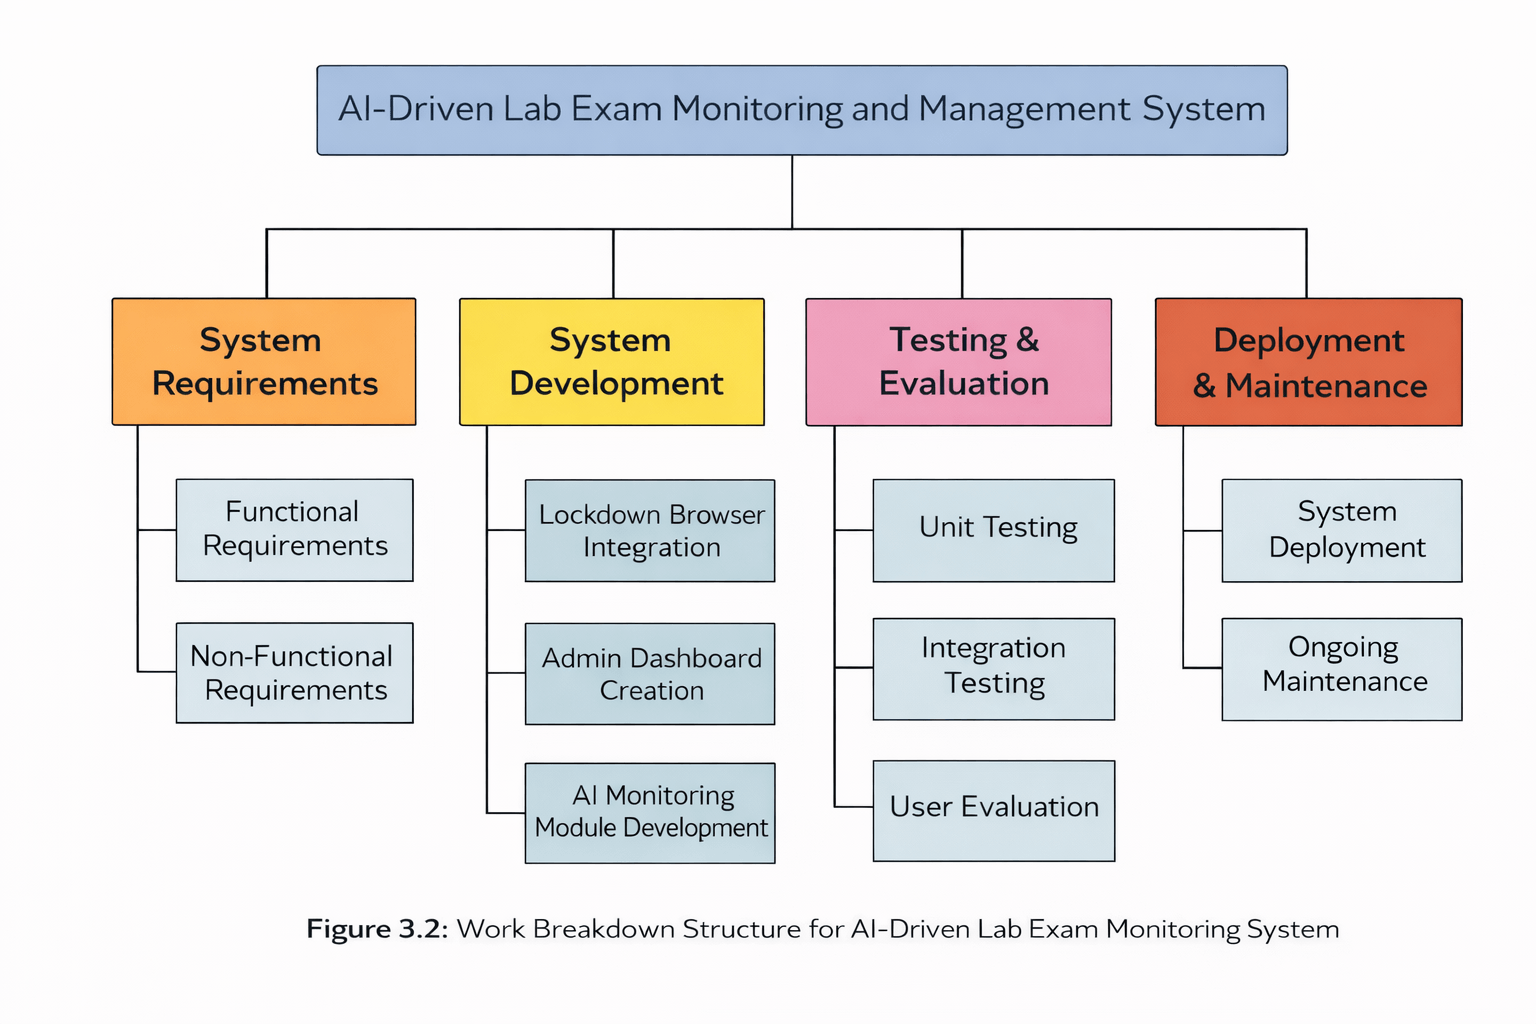
\includegraphics[width=0.95\linewidth]{Figures/work_breakdown_structure.png}
\caption{Work Breakdown Structure of the Proposed Project}
\label{fig:wbs}
\end{figure}

The WBS provides team members with clear scope responsibility. If a module appears in a sprint backlog, all team members understand which WBS node that module corresponds to, preventing double-handling and making scope creep immediately visible \cite{spp1}.

\subsection{Critical Path Method}

The Critical Path Method (CPM) identifies the sequence of tasks determining the shortest project duration \cite{spp1}. If any task on this critical path is delayed, it postpones the entire project's completion. Tasks not on the critical path possess slack, acting as buffers that allow schedule deviations without affecting the project completion date. This project is structured as a CPM network starting with Activity A (Gathering Requirements, 1 week) which has three dependent paths. Path 1 consists of Task B (Lockdown Client Development, 3 weeks) leading to Task E (AI Monitoring, 3 weeks). Path 2 comprises Task C (Admin Dashboard, 2 weeks) and Task D (Question Bank, 2 weeks), both feeding into Task G (Unit Testing, 1 week). Path 3 is Task F (Student Exam Client, 2 weeks). Tasks E, G, and F converge at Task H (System Integration Testing, 1 week) before ending with Task I (System Deployment, 1 week), as illustrated in Figure~\ref{fig:criticalpath}.

The critical path spans tasks A $\rightarrow$ B $\rightarrow$ E $\rightarrow$ H $\rightarrow$ I, with a total duration of 9 weeks (1+3+3+1+1). The slack along these critical tasks is zero, meaning any delay directly pushes back the deployment deadline. Path 2 tasks (C, D, G) have 1 week of slack, while Path 3 (Task F) has 4 weeks of slack, identifying them as resource-sourcing pools if critical tasks run behind.

\begin{figure}[H]
\centering

\includegraphics[width=0.95\linewidth]{Figures/critical_path.png}
\caption{Critical Path of the Proposed Project Activities}
\label{fig:criticalpath}
\end{figure}

\subsubsection{Schedule Control and Review}

SmartExam utilizes sprint burn-down charts rather than passive calendar checking \cite{scrum1}. At the end of each sprint, progress is evaluated against initial plans. If the percentage of completed story points falls below 80\%, up to a one-day recovery session is conducted before starting the next sprint, ensuring delays are identified early instead of surfacing only during the final integration sprint.
